\documentclass[12pt]{article}

% Layout.
\usepackage[top=1in, bottom=0.75in, left=1in, right=1in, headheight=1in, headsep=6pt]{geometry}

% Fonts.
\usepackage{mathptmx}
\usepackage[scaled=0.86]{helvet}
\renewcommand{\emph}[1]{\textsf{\textbf{#1}}}

% TiKZ.
\usepackage{tikz, pgfplots}
\usetikzlibrary{calc, arrows.meta}

% Misc packages.
\usepackage{amsmath,amssymb,latexsym}
\usepackage{graphicx}
\usepackage{array}
\usepackage{xcolor}
\usepackage{multicol}
\usepackage{fancyhdr}
\pagestyle{fancy}


% Misc.
\renewcommand{\d}{\displaystyle}
\newcommand{\ds}{\displaystyle}
\def\bc{\begin{center}}
\def\ec{\end{center}}
\def\be{\begin{enumerate}}
\def\ee{\end{enumerate}}

\newcommand{\ans}[1][1in]{\rule{#1}{.5pt}}


\lhead{Math F113X: Quiz 8}

\begin{document}

\vspace{1cm}

\noindent \textbf{Name:} \hrulefill \quad  score:\ans[1cm] \ / 10 \\


There are 10 points possible on this quiz. No aids (book, notes, etc.)
are permitted. You may use a non-programmable calculator.  {\bf Show
all work and supporting calculations for full credit. Explain how you
get your answers.}

\be

\item Consider the {\bf scheduling digraph} below.

\vspace{1cm}

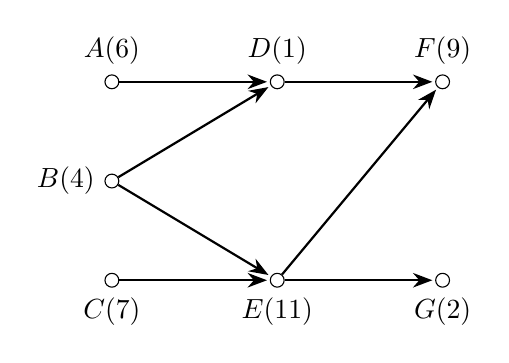
\begin{tikzpicture}[
    vertex/.style={circle, draw, fill=white, inner sep=0pt, minimum size=5pt},
    edge/.style={-{Stealth[length=7pt]}, thick, shorten >=1pt},
    x=3cm, y=1.8cm, scale=0.7]
  % Vertices
  \node[vertex, label=above:{$A(6)$}]  (A) at (0,2) {};
  \node[vertex, label=left:{$B(4)$}]   (B) at (0,1) {};
  \node[vertex, label=below:{$C(7)$}]  (C) at (0,0) {};
  \node[vertex, label=above:{$D(1)$}]  (D) at (1,2) {};
  \node[vertex, label=below:{$E(11)$}] (E) at (1,0) {};
  \node[vertex, label=above:{$F(9)$}]  (F) at (2,2) {};
  \node[vertex, label=below:{$G(2)$}]  (G) at (2,0) {};
  % Arcs
  \draw[edge] (A) -- (D);
  \draw[edge] (B) -- (D);
  \draw[edge] (B) -- (E);
  \draw[edge] (C) -- (E);
  \draw[edge] (D) -- (F);
  \draw[edge] (E) -- (F);
  \draw[edge] (E) -- (G);
\end{tikzpicture} \hfill
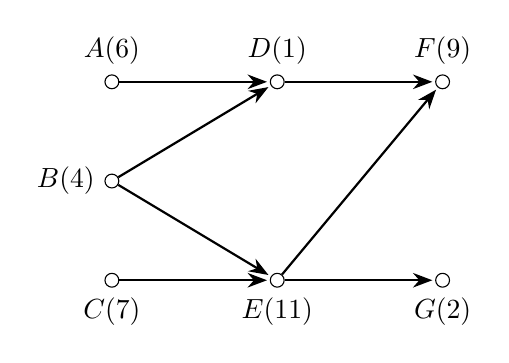
\begin{tikzpicture}[
    vertex/.style={circle, draw, fill=white, inner sep=0pt, minimum size=5pt},
    edge/.style={-{Stealth[length=7pt]}, thick, shorten >=1pt},
    x=3cm, y=1.8cm, scale=0.7]
  % Vertices
  \node[vertex, label=above:{$A(6)$}]  (A) at (0,2) {};
  \node[vertex, label=left:{$B(4)$}]   (B) at (0,1) {};
  \node[vertex, label=below:{$C(7)$}]  (C) at (0,0) {};
  \node[vertex, label=above:{$D(1)$}]  (D) at (1,2) {};
  \node[vertex, label=below:{$E(11)$}] (E) at (1,0) {};
  \node[vertex, label=above:{$F(9)$}]  (F) at (2,2) {};
  \node[vertex, label=below:{$G(2)$}]  (G) at (2,0) {};
  % Arcs
  \draw[edge] (A) -- (D);
  \draw[edge] (B) -- (D);
  \draw[edge] (B) -- (E);
  \draw[edge] (C) -- (E);
  \draw[edge] (D) -- (F);
  \draw[edge] (E) -- (F);
  \draw[edge] (E) -- (G);
\end{tikzpicture}

\vspace{1cm}

  \be
\item (2 points) Label the vertices in your scheduling digraph using the {\bf
    backflow algorithm}. Use square brackets $\left[ \, \, \right]$ for these
  labels. {\it A second copy of the digraph is provided in case you need to
  make corrections.} If you have labels on both digraphs, you must
  clearly label which one contains your final answer.
  \vspace{1cm}

\item (2 points) What priority list do you get if you prioritize the tasks using
  the {\bf critical path algorithm}?
  \ee

  \vfill
  
    \item (2 points) Suppose a particular schedule has a critical time of 28 hours and it takes one processor 65 hours to complete all the tasks. Is it possible for there to exist a schedule for two processors that uses only 28 hours? Explain your answer with some words or a computation.
  
  \vfill
  
  \newpage
  
(A tabula recta is at the end of this quiz.)

\item (2 points) Encrypt the message {\bf THANKSGIVING} using an alphabetic
  Caesar (shift) cipher with shift 4 (A to E).
  \vfill

\item (2 points) Decrypt the message {\bf KVUHT KFCA} using an alphabetic Caesar
  (shift) cipher with shift 2 (A to C).
  \vfill
  
\ee

\newpage

\vspace{1cm}

\begin{center}
{\Large  A Tabula Recta}
\end{center}



\vspace{.5in}

\makeatletter
\newcommand{\Letter}[1]{\@Alph{#1}}
\makeatother

\def\r{.6}
\hspace*{-.5in}
\begin{tikzpicture}
% "Plain Text" centered heading above the table columns
\path (14*\r+1*\r, 27*\r+0.55) node {\textbf{\Large{Plain Text}}};
\draw[step=\r] (0,0) grid (28*\r,27*\r);
\foreach \i in {1,2,...,26}{\path (\i*\r+1/2*\r +1*\r, 27*\r-1/2*\r) node {\textbf{\Letter{\i}}};}%
\foreach \i in {1,2,...,26}{\path (1/2*\r+1*\r, 26*\r-\i*\r+1/2*\r) node {\textbf{\Letter{\i}}};}%
\foreach \i in {1,2,...,26}{\path let \n1 = {int(\i-1)} in  (1/2*\r, 26*\r-\i*\r+1/2*\r) node {\n1};}%
\draw[line width = .75mm] (0,26*\r) -- (28*\r, 26*\r);
\draw[line width = .75mm] (\r+1*\r,0) -- (\r+1*\r, 27*\r);
% "Cipher text Shift" vertical label on the left, reading bottom to top
\node[rotate=90] at (-0.45, 13*\r) {\textbf{\Large{Cipher text Shift}}};
\foreach \i in {1,2,...,26}
	\foreach \j in {1,2,...,26}{
		{\path let \n1 = {int(mod((\j-1)+(\i-1), 26)+1} in (\i*\r+1/2*\r+1*\r, 27*\r-\j*\r - 1/2*\r) node {\Letter{\n1}};
		}}
\end{tikzpicture}


\end{document}
%%% Local Variables:
%%% mode: LaTeX
%%% TeX-master: t
%%% End:
